\section{Existing prototype}
\label{sec:existing_prototype}


\subsection{Structure}
class diagram

organisation

vs solution


\subsection{Data structure}
\label{sec:data_structure}

regular grid

macro/micro cells

triangles in cells, pointer to sweep volumes


\subsection{Classification}

description of classification algorithm (principle)

images from RISC presentation

\begin{figure}
\centering
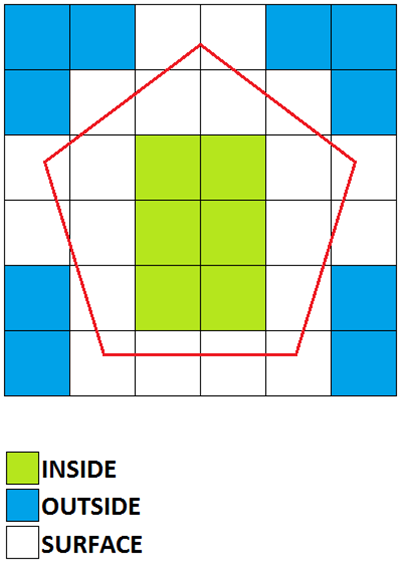
\includegraphics[width=0.4\linewidth]{classification}
\caption{Principle of classifying cells of the grid.}
\label{fig:classification}
\end{figure}

\begin{figure}
\centering
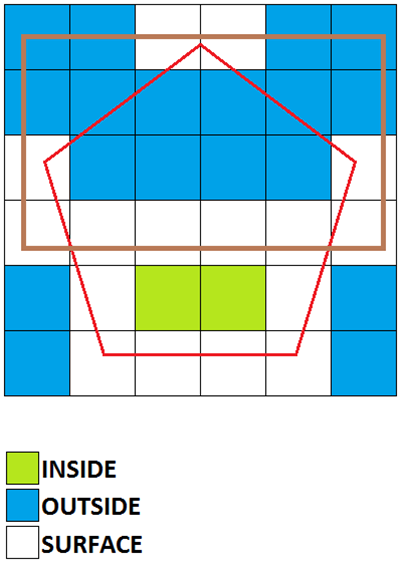
\includegraphics[width=0.4\linewidth]{classification_sub}
\caption{Classification result after adding a subtraction volume. }
\label{fig:classification_sub}
\end{figure}

\subsection{Adapted raycasting algorithm}

consequences of classification on raycasting algorithm

implicit geometry, water tightness? why no problem?

algorithm description of CPU caster
